\documentclass[10pt]{beamer}

\usepackage{fontspec}
\usepackage{polyglossia}
\usepackage{xgreek}

\setdefaultlanguage{greek}
\setotherlanguages{english}
\setmainfont[Kerning=On]{Linux Libertine O}
\setsansfont[Kerning=On]{Linux Libertine O}
\setromanfont[Kerning=On]{Linux Libertine O}
\newfontfamily\greekfont[Script=Greek]{Linux Libertine O}
\newfontfamily\greekfontsf[Script=Greek]{Linux Libertine O}
\newfontfamily{\greekfonttt}{Linux Libertine O}

\usepackage{diagbox}
\usepackage{multirow,rotating}
\usepackage{color}
\usepackage{tikz-cd}
\usepackage{array}
\usepackage{siunitx}
\usepackage{mathtools,nccmath}%
\usepackage{etoolbox, xparse}
\usetheme{CambridgeUS}
\usecolortheme{dolphin}
\usepackage[
    n,
    operators,
    advantage,
    sets,
    adversary,
    landau,
    probability,
    notions,
    logic,
    ff,
    mm,
    primitives,
    events,
    complexity,
    asymptotics,
    keys]{cryptocode}

\definecolor{myNewColorA}{RGB}{158, 27,50}
\definecolor{myNewColorB}{RGB}{158, 27,50}
\definecolor{myNewColorC}{RGB}{158, 27,50}
\setbeamercolor*{palette primary}{bg=myNewColorC}
\setbeamercolor*{palette secondary}{bg=myNewColorB, fg = white}
\setbeamercolor*{palette tertiary}{bg=myNewColorA, fg = white}
\setbeamercolor*{titlelike}{fg=myNewColorA}
\setbeamercolor*{title}{bg=myNewColorA, fg = white}
\setbeamercolor*{item}{fg=myNewColorA}
\setbeamercolor*{caption name}{fg=myNewColorA}
\definecolor{mygray}{rgb}{0.4,0.4,0.4}
\definecolor{mygreen}{rgb}{0,0.8,0.6}
\definecolor{myorange}{rgb}{1.0,0.4,0}
\definecolor{light-gray}{gray}{0.80}
\usefonttheme{professionalfonts}
\usepackage{hyperref}
\usepackage{minted}
\usepackage{listings}

\titlegraphic{%
    
\includegraphics[width=3.0cm]{logo.png}
}

\setbeamerfont{title}{size=\large}
\setbeamerfont{subtitle}{size=\small}
\setbeamerfont{author}{size=\small}
\setbeamerfont{date}{size=\footnotesize}
\setbeamerfont{institute}{size=\footnotesize}
\title[Μελέτη Πρωτοκόλλων Ασφαλούς Υπολογισμού Πολλών Μερών]{Μελέτη Πρωτοκόλλων Ασφαλούς Υπολογισμού Πολλών Μερών \\ (Study on Secure Multi Party Computation Protocols)}%title
\author[Θεόδωρος Συμεωνίδης Α.Μ. 1064870]{Θεόδωρος Συμεωνίδης \\ Α.Μ. 1064870}

\institute[]{Τμήμα Μηχανικών Η/Υ και Πληροφορίκής \\ Πανεπιστήμιο Πατρών}
\date[\textcolor{white}{Τμήμα Μηχανικών Η/Υ και Πληροφορικής}]
{\today}

\AtBeginSection[]{
    \begin{frame}
        \vfill
        \centering
        \begin{beamercolorbox}[sep=8pt,center,shadow=true,rounded=true]{title}
            \usebeamerfont{title}\insertsectionhead\par%
        \end{beamercolorbox}
        \vfill
    \end{frame}
}

\lstset{language=C++,
    basicstyle=\footnotesize\sffamily\color{black},
    commentstyle=\color{mygray},
    numbers=left,
    numbersep=5pt,
    numberstyle=\tiny\color{mygray},
    keywordstyle=\color{mygreen},
    showspaces=false,
    showstringspaces=false,
    stringstyle=\color{myorange},
    tabsize=2
}

\usepackage[natbib=true,style=authoryear,backend=bibtex,useprefix=true]{biblatex}
\addbibresource{../shortbibliography.bib}

\begin{document}

    \begin{frame}
        \titlepage
    \end{frame}

    \section{Εισαγωγή}
    \begin{frame}{Εισαγωγή}
        \begin{block}{}
            Το αντικείμενο αυτής της διπλωματικής εργασίας :
            \begin{itemize}
                \item Μελέτη Πρωτοκόλλων Ασφαλούς Υπολογισμού Πολλών Μερών (Secure Multi Party Computation (SMPC) Protocols)
                \item Εφαρμογή τους στην κατασκευή μιας Ασφαλούς Υπολογισμού Δύο Μερών BLAS Level-1 Βιβλιοθήκης, για πρώτη φορά στη βιβλιογραφία
            \end{itemize}
        \end{block}
        \begin{block}{}
            Για να επιτευχθεί το παραπάνω έγινε εισαγωγή και αναπτύχθηκε το εξής θεωρητικό υπόβαθρο :
            \begin{itemize}
                \item Μαθηματικά της κρυπτογραφίας
                \item Σύγχρονα κρυπτογραφικά εργαλεία που χρησιμοποιούνται σε πρωτόκολλα SMPC
                \item Θεωρητικά αποδείξιμη ασφάλεια
            \end{itemize}
        \end{block}
    \end{frame}

    \begin{frame}{Εισαγωγή}
        \begin{block}{}
            \textbf{Ασφαλής Υπολογισμός} : Όλες οι υπολογιστικές μέθοδοι που επιτρέπουν τον υπολογισμό επάνω σε δεδομένα κρατώντας τα δεδομένα μυστικά. Τα δεδομένα, δηλαδή, ένα μέρος των δεδομένων μπορεί να ανήκουν σε κάποιον τρίτο ο οποίος δε θέλει να μας φανερώσει τις τιμές τους.
        \end{block}{}
        \begin{block}{}
            Παραδείγματα :
            \begin{itemize}
                \item Υπολογισμός του εσωτερικού γινομένου δυό διανυσμάτων από ένα άτομο ενώ τα διανύσματα παρέχονται από κάποιο άλλο άτομο. Το πρώτο άτομο μπορεί να υπολογίσει το αποτέλεσμα χωρίς να μάθει τις πραγματικές τιμές των διανυσμάτων αυτών του δεύτερου ατόμου.
                \item Υπολογισμός της Ευκλείδιας Νόρμας ενός διανύσματος από το οποίο κάθε άτομο μιας ομάδας άτομο διαθέτει ένα στοιχείο
            \end{itemize}
        \end{block}
        \begin{block}{}
            \textbf{Επαληθεύσιμος Υπολογισμός} : Όλες οι υπολογιστικές μέθοδοι που επιτρέπουν την επαλήθευση πως η έξοδος του υπολογισμού που εξήγαγαν είναι πράγματι η έξοδος του υπολογισμού και των δεδομένων που τους δόθηκαν.
        \end{block}{}
    \end{frame}

    \begin{frame}{Εισαγωγή}
        \begin{block}{}
            \textbf{Κατηγορίες Ασφαλούς και Επαληθεύσιμου Υπολογισμού}
            \begin{itemize}
                \item Ασφαλής Αναθέσιμος Υπολογισμός : Μη διαδραστικά πρωτόκολλα υπολογισμού (π.χ. HE, SWHE, FHE)
                \item \textbf{Ασφαλής Υπολογισμός Πολλών Μερών} : Διαδραστικά πρωτόκολλα υπολογισμού
            \end{itemize}
        \end{block}
    \end{frame}

    \section{Ασφαλής Υπολογισμός Πολλών Μερών \\ (Secure Multi Party Computation (SMPC))}
    \begin{frame}
        \begin{block}{}
            \textbf{Ασφαλής Υπολογισμός Πολλών Μερών (Secure Multi Party Computation ή SMPC)} : Είναι μια κλάση διαδραστικών κρυπτογραφικών σχημάτων που επιτρέπουν σε συμμετέχοντες $P_1, P_2, \dots, P_n$ με αντίστοιχες εισόδους $x_1, x_2, \dots, x_n$ να υπολογίσουν τη συνάρτηση την έξοδο $y$ της συνάρτησης $f$, ως $y = f(x_1, x_2, \dots, x_n)$ και ικανοποιούν τις παρακάτω ιδιότητες :
            \begin{itemize}
                \item Ορθότητα : Η έξοδος $y$ είναι η σωστή έξοδος της συνάρτησης για τις δεδομένες εισόδους
                \item Ιδιωτικότητα : Η έξοδος $y$ είναι η μόνη πληροφορία που φανερώνει το πρωτόκολλο σε έναν αντίπαλο που ελέγχει κάποιους διεφθαρμένους συμμετέχοντες.
            \end{itemize}
        \end{block}
    \end{frame}

    \begin{frame}
        \begin{block}{}
            \textbf{Εφαρμογές Ασφαλούς Υπολογισμού Πολλών Μερών} :
            \begin{itemize}
                \item Κατανεμημένες ψηφοφορίες και ιδιωτικές ψήφους
                \item Μηχανική Μάθηση που Διατηρεί την Ιδιωτικότητα (Privacy Preserving Machine Learning)
                \item Στατιστική που Διατηρεί την Ιδιωτικότητα (Privacy Preserving Statistics)
                \item Ψηφιακές Υπογραφές Κατωφλίου (Threshold Digital Signatures) με μοναδικό ιδιωτικό κλειδί το οποίο διανέμεται σε κατάλληλη μορφή στους συμμετέχοντες ώστε αν ο κατάλληλος αριθμός συμμετεχόντων συνεργαστεί να μπορεί να παράξει μια υπογραφή χωρίς να χρειάζεται να ανακατασκευαστεί το κλειδί.
            \end{itemize}
        \end{block}
    \end{frame}

    \begin{frame}[c]{}
        \centering
        \begin{block}{}
            \textbf{Κατηγορίες SMPC πρωτοκόλλων ως προς το μοντέλο αναπαράσταση του υπολογισμού} :
            \begin{itemize}
                \item Αναπαράσταση ως Boolean δίκτυο/κύκλωμα Συνδυαστικής Λογικής
                \item Αναπαράσταση ως Αριθμητικό δίκτυο/κύκλωμα
                \item Πιο σύνθετες αναπαραστάσεις, όπως ως Μηχανή Turing ή RAM (Random Access Machine)
            \end{itemize}
        \end{block}
    \end{frame}

    \begin{frame}[c]{}
        \centering
        \begin{block}{}
            \textbf{Κατηγορίες πρωτοκόλλων SMPC ως προς τις ιδιότητες ασφάλειας} :
            \begin{itemize}
                \item Πρωτόκολλα ασφαλή ενάντια σε Παθητικούς Αντιπάλους
                \begin{itemize}
                    \item Ασφαλή ενάντια σε διεφθαρμένη μειοψηφία
                    \item Ασφαλή ενάντια σε διεφθαρμένη πλειοψηφία
                \end{itemize}
                \item Πρωτόκολλα ασφαλή ενάντια σε Ενεργητικούς Αντιπάλους
                \begin{itemize}
                    \item Ασφαλή ενάντια σε διεφθαρμένη μειοψηφία
                    \item Ασφαλή ενάντια σε διεφθαρμένη πλειοψηφία
                \end{itemize}
            \end{itemize}
        \end{block}
    \end{frame}

    \begin{frame}[fragile,c]{}
        \begin{block}{}
            \begin{table}[h!]
                \centering
                \resizebox{\columnwidth}{!}{
                    \begin{tabular}{|c|l|ll|ll|}
                        \hline
                        \multicolumn{1}{|l|}{}       &                                                                      & \multicolumn{2}{c|}{Αριθμητικό δίκτυο}                                    & \multicolumn{2}{c|}{Boolean κύκλωμα}                                 \\ \hline
                        \multicolumn{1}{|l|}{}       & \diagbox{Μοντέλο Ασφάλειας}{Υπολογιστικό Μοντέλο} & \multicolumn{1}{l|}{$modp$ ή $GF(2^n)$}          & $mod2^n$               & \multicolumn{1}{l|}{Δυαδική Διαμοίραση Μυστικών} & Μπερδεμένα Δίκτυα \\ \hline
                        \multirow{}{}{Ενεργη\-τικός}   & Διεφθαρμένη Πλειοψηφία                                               & \multicolumn{1}{l|}{MASCOT / LowGear / HighGear} & SPDZ2k                 & \multicolumn{1}{l|}{Tiny / Tinier}               & BMR               \\ \cline{2-6}
                        & Εμπιστή Πλειοψηφία                                                   & \multicolumn{1}{l|}{Shamir / Rep3 / PS / SY}     & Brain / Rep3 / PS / SY & \multicolumn{1}{l|}{Rep3 / CCD / PS}             & BMR               \\ \cline{2-6}
                        & Έμπιστη Υπερ-πλειοψηφία                                              & \multicolumn{1}{l|}{Rep4}                        & Rep4                   & \multicolumn{1}{l|}{Rep4}                        & N/A               \\ \hline
                        Συγκαλλημένος                       & Διεφθαρμένη Πλειοψηφία                                               & \multicolumn{1}{l|}{CowGear / ChaiGear}          & N/A                    & \multicolumn{1}{l|}{N/A}                         & N/A               \\ \hline
                        \multirow{}{}{Παθη\-τικός} & Διεφθαρμένη Πλειοψηφία                                               & \multicolumn{1}{l|}{Semi / Hemi / Temi / Soho}   & Semi2k                 & \multicolumn{1}{l|}{SemiBin}                     & Yao's GC / BMR    \\ \cline{2-6}
                        & Έμπιστη Πλειοψηφία                                                   & \multicolumn{1}{l|}{Shamir / ATLAS / Rep3}       & Rep3                   & \multicolumn{1}{l|}{Rep3 / CCD}                  & BMR               \\ \cline{2-6}
                        & Dealer                                                               & \multicolumn{1}{l|}{Dealer}                      & Dealer                 & \multicolumn{1}{l|}{Dealer}                      & N/A               \\ \hline
                    \end{tabular}
                }
                \caption{Παράδειγμα υποστηριζόμενων πρωτοκόλλων της βιβλιοθήκης MP-SPDZ. Ο παρόν είναι εμπνευσμένος από έναν παρόμοιο, αλλά δυσανάγνωστο, πίνακα που υπάρχει στα εγχειρίδια χρήσης της.}
                \label{fig:mp-sdpz-protocols}
            \end{table}
        \end{block}
    \end{frame}
    \begin{frame}{Πρωτόκολλο GMW}
        \begin{block}{}
            \begin{itemize}
                \item Προτάθηκε από τους Goldreich, Micali, Wigderson το 1987
                \item Βασίζεται σε Δυαδική Διαμοίραση Μετοχών
                \item Είναι ασφαλές ενάντια σε παθητικούς αντιπάλους
                \item Μπορεί να χρησιμοποιηθεί για $n \ge 2$ συμμετέχοντες
                \item Μπορεί να εκτελέσει Boolean και Αριθμητικά κυκλώματα
                \item Οι Boolean πύλες NOT και XOR μπορούν να αποτιμηθούν, μη διαδραστικά
                \item Η Boolean πύλη AND απαιτεί διάδραση για την αποτίμηση της.
            \end{itemize}
        \end{block}
    \end{frame}

    \begin{frame}{Πρωτόκολλο GMW}
        \begin{block}{}
            Θα εξετάσουμε την περίπτωση δύο συμμετεχόντων, $P_1$ και $P_2$, και μιας Boolean πύλης με δύο bit εισόδου και ένα bit εξόδου :
            \begin{itemize}
                \item \textbf{Πύλη εισόδου} : Έστω πως ο συμμετέχον $P_1$ διαθέτει ένα ιδιωτικό bit εισόδου $x_i$ το οποίο αντιστοιχεί σε ένα καλώδιο $w_i$ του κυκλώματος. Έστω επίσης $s_i^j$ η μετοχή για το καλώδιο $w_i$ του παίχτη $j$. Για κάθε καλώδιο $i$ επιθυμούμε $s_i^j \oplus s_i^{j-1} = w_i$. Ο $P_1$ δημιουργεί τις μετοχές ως εξής :
                \begin{itemize}
                    \item Στέλνει στον $P_2$ το $r_i \sample \bin$, η οποία είναι η μετοχή του $P_2$ για το καλώδιο $w_i$, $s_i^2 = r_i$
                    \item Δημιουργεί τη δική του μετοχή του $w_i$ ως εξής : $s_i^1 = x_i \oplus r_i$
                \end{itemize}
                \item \textbf{Πύλη NOT} : Έστω το καλώδιο εισόδου $w_k$ και το καλώδιο εξόδου $w_{k+1}$. Στην περίπτωση της Πύλης NOT, ένας από τους δύο συμμετέχοντες (όχι και οι δύο), έστω ο $P_1$, το μόνο που έχει να κάνει είναι να αντιστρέψει το bit της μετοχής του, δηλαδή $s_{k+1}^1 = 1-s_k^1$
                \item \textbf{Πύλη XOR} : Έστω τα καλώδια εισόδου $w_k$, $w_{k+1}$ και το καλώδιο εξόδου $w_{k+2}$. Στην περίπτωση της Πύλης XOR, οι δύο συμμετέχοντες κάνουν XOR τις μετοχές που έχουν για κάθε μία από τις δύο εισόδους της πύλης. Δηλαδή $s_{k+2}^1 = s_{k}^1 \oplus s_{k+1}^1$ και $s_{k+2}^2 = s_k^2 \oplus s_{k+1}^2$
            \end{itemize}
        \end{block}
    \end{frame}

    \begin{frame}{Πρωτόκολλο GMW}
        \begin{block}{}
            \begin{itemize}
                \item \textbf{Πύλη AND}: Έστω τα καλώδια εισόδου $w_k$, $w_{k+1}$ και το καλώδιο εξόδου $w_{k+2}$. Στην περίπτωση της Πύλης AND, ο ένας από τους δύο συμμετέχοντες, έστω ο $P_1$ πρέπει να ετοιμάσει ένα 1-4 ΟΤ της παρακάτω συνάρτησης :
                $$
                S=S_{s_i^1, s_j^1}\left(s_i^2, s_j^2\right)=\left(s_i^1 \oplus s_i^2\right) \wedge\left(s_j^1 \oplus s_j^2\right)
                $$
                Αυτό το κάνει επιλέγοντας $r \sample \bin$ και στη συνέχεια δημιουργόντας τον παρακάτω πίνακα από τον οποία στέλνει την κατάλληλη γραμμή μέσω 1/4 OT ανάλογα με το τι τιμή έχουν οι μετοχές του $P_2$ :
                $$
                T_G=\left(\begin{array}{l}
                              r \oplus S(0,0) \\
                              r \oplus S(0,1) \\
                              r \oplus S(1,0) \\
                              r \oplus S(1,1)
                \end{array}\right)
                $$
            \end{itemize}
        \end{block}
    \end{frame}

    \section{BLAS (Basic Linear Algebra Subroutines)}
    \begin{frame}
        \begin{block}{}
            \textbf{BLAS} : Είναι μια διεπαφή/πρότυπο συναρτήσεων και ρουτινών γραμμικής που επιτρέπει σε έναν κατασκευαστή υλικού να δημιουργήσει μια δική του υλοποίηση του προτύπου είναι παραμετροποιημένη για το συγκεκριμένο υλικό. Χωρίζεται σε τρία επίπεδα.
            \begin{itemize}
                \item Level-1 : Πράξεις μεταξύ διανυσμάτων
                \item Level-2 : Πράξεις πινάκων με διανύσματα
                \item Level-3 : Πράξεις μεταξύ πινάκων
            \end{itemize}
        \end{block}
        \begin{block}{}
            H διεπαφή της BLAS υπάρχει για δύο γλώσσες προγραμματισμού :
            \begin{itemize}
                \item FORTAN και αποκαλείται BLAS
                \item \textbf{C/C++ και αποκαλείται CBLAS}
            \end{itemize}
            Η BLAS διεπαφή χρησιμοποιείται σχεδόν από κάθε πρόγραμμα που κάνει πράξεις γραμμικής άλγεβρας, ενδεικτικά αναφέρουμε τα εξής :
            \begin{itemize}
                \item Βιβλιοθήκες επιστημονικού υπολογισμού όπως η NumPy και η Sci-Py
                \item Βιβλιοθήκες μηχανικής μάθησης όπως η Tensorflow και η PyTorch
                \item Προγράμματα επιστημονικού υπολογισμού όπως το MATLAB
            \end{itemize}
        \end{block}
    \end{frame}

    \begin{frame}[fragile]{Παραδείγματα προτύπου CBLAS}

        \begin{block}{}
            \begin{lstlisting}[firstnumber=1, xleftmargin=10pt, language=C++]
float  cblas_sdot(const CBLAS_INT N,
                  const float  *X, const CBLAS_INT incX,
                  const float  *Y, const CBLAS_INT incY);
            \end{lstlisting}
        \end{block}
        \begin{block}{}
            \begin{lstlisting}[firstnumber=1, xleftmargin=10pt, language=C++]
void cblas_saxpy(const CBLAS_INT N,
                 const float alpha,
                 const float *X, const CBLAS_INT incX,
                 float *Y, const CBLAS_INT incY);
            \end{lstlisting}
        \end{block}

    \end{frame}

    \section{Περιγραφή προβλήματος}
    \begin{frame}[c]{}
        \centering
        \begin{block}{}
            Οι BLAS βιβλιοθήκες χρησιμοποιούνται σχεδόν παντού, από τον Επιστημονικό Υπολογισμό μέχρι την Μηχανική Μάθηση κσι σε τομείς που η ιδωτικότητα των επεξεργαζόμενων δεδομένων είναι ιδιαίτερα επιθυμητή. Ωστόσο, δεν υπάρχει στη βιβλιογραφία, τουλάχιστον στη δική μας γνώση, κάποια βιβλιοθήκη που να επιτρέπει τη χρήση BLAS συναρτήσεων για Ασφαλή Υπολογισμό Πολλών Μερών και να μπορεί να λειτουργήσει ως σχεδόν drop-in αντικατάστατο μιας κανονικής βιβλιοθήκης.
        \end{block}
    \end{frame}

    \section{Επίλυση προβλήματος}
    \begin{frame}[c]{}
        \centering
        \begin{block}{}
            Εφαρμογή του SMPC πρωτοκόλλου GMW στην κατασκευή της βιβλιοθήκης MPC-BLAS, μιας Ασφαλούς Υπολογισμού Δύο Μερών BLAS Level-1 βιβλιοθήκης, η οποία κατά τη γνώση μας, παρουσιάζεται πρώτη φορά στη βιβλιογραφία.
        \end{block}
    \end{frame}

    \begin{frame}{Η βιβλιοθήκη MPC-BLAS}
        \textbf{Περιγραφή} :
        \begin{itemize}
            \item Ένα πρόγραμμα που είναι χρησιμοποιεί τη διεπαφή CBLAS απαιτεί ελάχιστες αλλαγές στον πηγαίο του κώδικα για να χρησιμοποιήσει την διεπαφή MPC-BLAS
            \item Απαιτεί δύο διεργασίες, μία για κάθε συμμετέχοντα οι οποίες μπορούν να τρέχουν στο ίδιο μηχάνημα ή σε διαφορετικό
            \item Υποστηρίζει μόνο το λειτουργικό σύστημα Linux, διότι είναι το μοναδικό που υποστηρίζεται από την βιβλιοθήκη ABY. Έχει αναπτυχθεί και ελεγχθεί σε Ubuntu 22.04 LTS
            \item Υλοποιεί όλες τις Level-1 BLAS ρουτίνες εκτός από τις xROTx, διότι η βιβλιοθήκη ABY έχει πολύ περιορισμένη υποστήριξη για πράξεις πινάκων.
        \end{itemize}
    \end{frame}

    \begin{frame}{Η βιβλιοθήκη MPC-BLAS}
        \textbf{Τεχνικές Προδιαγραφές} :
        \begin{itemize}
            \item Γραμμένη σε C++20 και χτισμένη με CMake
            \item Βασισμένη στην βιβλιοθήκη ABY για τις κρυπτογραφικές πράξεις και την εκτέλεση του πρωτοκόλλου GMW.
            \item Απαιτεί στατική σύνδεση (static linking), λόγω περιορισμών της βιβλιοθήκης ABY
        \end{itemize}
    \end{frame}

    \begin{frame}[fragile]{Προσαρμογή προγράμματος από CBLAS σε MPC-BLAS 1}
        \begin{columns}[c] % align columns
            \begin{column}{.48\textwidth}
                \begin{block}{}
                    \begin{lstlisting}[firstnumber=1, xleftmargin=5pt, basicstyle=\footnotesize, language=C++]
float result_1 =
    cblas_sdot(4,
               test_vector_1,1,
               test_vector_2,1);
                    \end{lstlisting}
                \end{block}
            \end{column}
            \hfill
            \begin{column}{.48\textwidth}
                \begin{block}{}
                    \begin{lstlisting}[firstnumber=1, xleftmargin=5pt, basicstyle=\footnotesize, language=C++]
mpcblas_initialize(SERVER,
                  "127.0.0.1",
                  7766,
                  bitlen);

float result_1 =
    mpcblas_sdot(4,
                 test_vector_1,1,
                 MPCBLAS_IGNORE,1)
            ->get_value();

mpcblas_uninitialize();
                    \end{lstlisting}
                \end{block}
            \end{column}%
        \end{columns}
    \end{frame}

    \begin{frame}[fragile]{Προσαρμογή προγράμματος από CBLAS σε MPC-BLAS 2}
        \begin{columns}[c]
            \begin{column}{.48\textwidth}
                \begin{block}{}
                    \begin{lstlisting}[firstnumber=1, xleftmargin=5pt, basicstyle=\footnotesize, language=C++]
cblas_saxpy(4,
    cblas_sdot(4,
               test_vector_1,1,
               test_vector_2,1),
            test_vector_1,1,
            test_vector_2,1);
float result =
    cblas_snrm2(4,
               test_vector_2,1);
                    \end{lstlisting}
                \end{block}
            \end{column}
            \hfill
            \begin{column}{.48\textwidth}
                \begin{block}{}
                    \begin{lstlisting}[firstnumber=1, xleftmargin=5pt, basicstyle=\footnotesize, language=C++]
mpcblas_initialize(CLIENT,
                   "127.0.0.1",
                    7766,
                    bitlen);
auto result y =
mpcblas_saxpy(4,
    mpcblas_sdot(4,
                 MPCBLAS_IGNORE,1,
                 test_vector_2,1),
              MPCBLAS_IGNORE,1,
              test_vector_2,1);
float result_2 =
    mpcblas_snrm2(4, y, 1)
            ->get_value();
mpcblas_uninitialize();
                    \end{lstlisting}
                \end{block}
            \end{column}%
        \end{columns}
    \end{frame}

    \begin{frame}[fragile, c]{Πείραμα}
        \begin{center}
            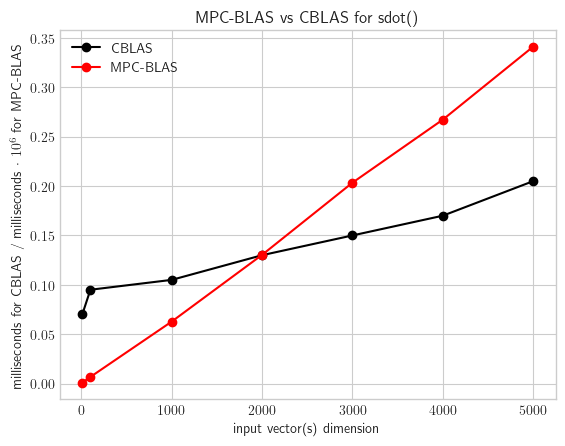
\includegraphics[scale=0.7]{./images/mpc-blas-timings-graph}
        \end{center}
    \end{frame}

    \begin{frame}{Ερμηνεία Πειράματος}
        \begin{block}{}
            \begin{itemize}
                \item Η επιβάρυνση που εισάγεται από τη χρήση της MPC-BLAS σε σύκριση με την CBLAS είναι γραμμική και είναι της τάξης των 10.000-100.000 χρονικών μονάδων
                \item Η διαφορά των χρονικών ασυμπτωτικών πολυπλοκοτήτων των δύο βιβλιοθηκών είναι σταθερή τιμή
                \item Υπάρχει τεράστιο περιθώριο βελτίωσης, ίσως και κατά αρκετές τάξεις μεγέθους
            \end{itemize}
        \end{block}

    \end{frame}

    \begin{frame}{Μελλοντική Μελέτη}
        \begin{block}{}
        \begin{itemize}
            \item Υλοποίηση των BLAS-2 και BLAS-3 υπορουτινών και ολοκλήρωση μιας εύχρηστης βιβλιοθήκης
            \item Υλοποίηση αποδοτικότερου αλγορίθμου Κινητής Υποδιαστολής (χρήση αριθμητικών δικτύων αντί για Boolean)
            \item Επέκταση της ABY για SMPC ή χρήση βιβλιοθήκης για υποστήριξη SMPC
            \item Επέκταση της ABY ή χρήση βιβλιοθήκης με υποστήριξη πρωτοκόλλων ασφαλών ενάντια σε Ενεργητικούς Αντιπάλους
        \end{itemize}
            \end{block}
    \end{frame}

    \begin{frame}[t,allowframebreaks]
        \nocite{*}
        \frametitle{Βιβλιογραφία}
        \printbibliography
    \end{frame}

    \begin{frame}[c]{Τέλος}
        \centering
        Τέλος \\[20pt]
        Ευχαριστώ
    \end{frame}

%    \section{Βιβλιογραφία}
%    \begin{frame}
%
%    \end{frame}
\end{document}
